\ifx \allfiles \undefined
\documentclass{article}
\usepackage{booktabs}
\usepackage{multirow}
\usepackage{graphicx}
\usepackage{subfigure}

\begin{document}
\title{Discuss}
\maketitle \else \fi

%\subsubsection{Who follows whom on twitter?}
%Table 1 shows the average numbers of followings in different universities with respect to users in different universities. 'Other' represents that the user does not mention any of these four universities in his biography. For example, the third row and second column means 38.17 followings of a UCLA user is in other universities on average. It is shown that the number of followers in the same university is ten times larger than that in different universities. However, this only counts for 5\% among all a user's followers. A possible reason might be that many users do not write their universities in their biographies.

\section{Discussion}\label{sec:discussion}
During our manually labeling process, we find several interesting results reflected by our algorithms. We distributed top 100 users of UCLA category returned by different algorithms into several categories and described phenomenons as follows.

\subsection{User classification}
The users are classified into $5$ types manually, they are active users in UCLA with related bio, tweets or photos (ActiveUCLA); inactive users in UCLA (InactiveUCLA); inactive users not belongs to UCLA (Inactive); user intent miss match (Intent); and active user not belongs to UCLA (Negative). The classification result is in Figure \ref{fig:userclass}.

\begin{figure}[h]
\centering
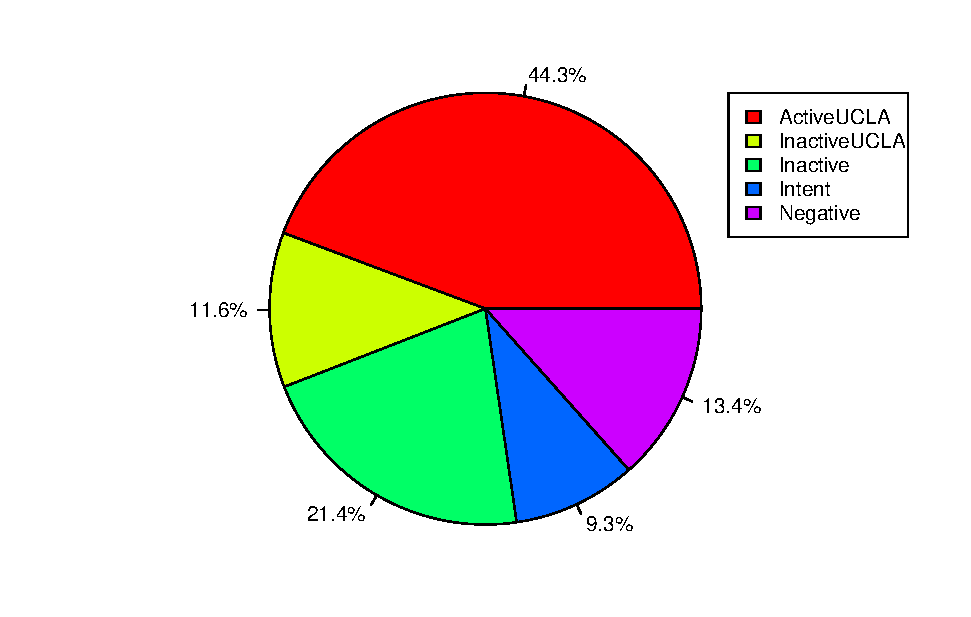
\includegraphics[width=0.5\textwidth]{experiment/uc.eps}
\caption{Manually user classification result.}
\label{fig:userclass}
\end{figure}

For active users, it is easy to see whether the user has related tweets about UCLA or photos about UCLA. For users without new tweets in recent two months, we call them inactive users and predict whether they are belong to UCLA category according to search result in Google. We type their names with UCLA and see whether there is related search results in top 10 positions.

\subsection{Intent mismatch}
The intent mismatch, labeled as ``Intent'' in Figure \ref{fig:userclass}, refers to the situations where the users are somehow interested in UCLA but it is actually not belong to UCLA. The data show that intent mismatch often arises when a user follows a lot of UCLA users or a user talks about something that mentions UCLA.

There are several examples of intent mismatch. First, users may follow UCLA members in order to have more business opportunities, such as ``WeTutorLA'' and ``bombaybite''. The former one follows lot of students from UCLA, USC, UCSD and so on to let them noticed. The latter one follows a lot of organizations of UCLA because it is a restaurant near UCLA. Second, some users keeps follow back a lot of users, such as ``0neNiteStan''. This kind of users have a lot of tweets for advertisement. Third, users like ``USCTrojansNews'', ``openwestwood'' would ranked at higher position in our result. These users' tweets have significant intersection with tweets generated by users from UCLA. For example, ``USCTrojansNews'' often publish tweets that compare UCLA with USC while some users in UCLA category also like to do that. This makes our model make mistakes during the training process.

These kinds of intent mismatch contribute to $9.3\%$ discrepancies in the data. Typically, intent mismatch are very hard to be corrected since it requires human understanding of why this user may related to target category but not belongs to that category.

\subsection{Precision of active user}

Noticed that there are about $30\%$ users are inactive users. Those users published several tweets after they register and didn't publish any more tweets during recent three months. In real cases, we don't want to see these inactive users since we don't expect that they will provide more information or business opportunity in the future. So that we evaluate our different approaches with inactive user as a negative example and the result is in Figure \ref{fig:activeprecision}.

\begin{figure}[h]
\centering
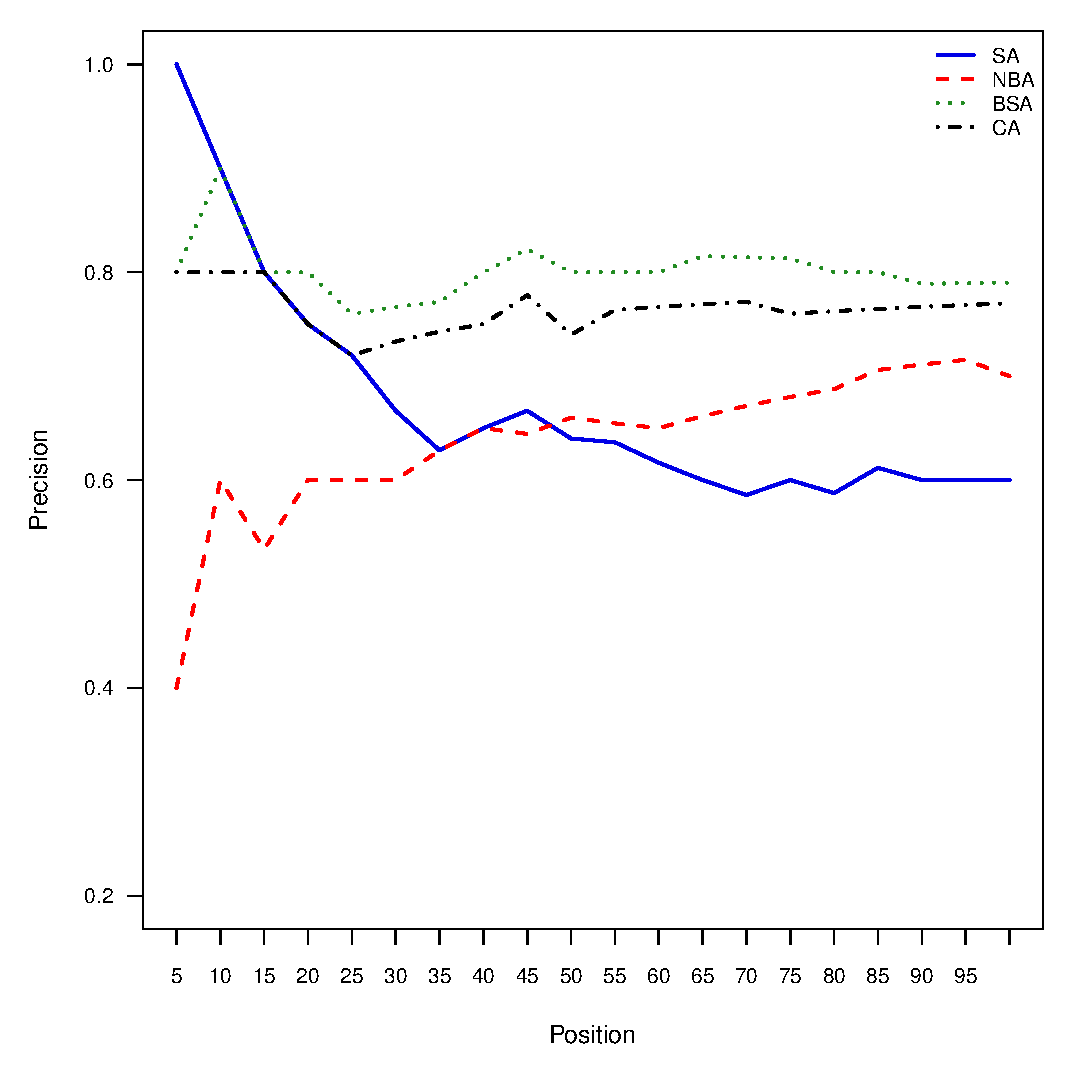
\includegraphics[width=0.45\textwidth]{experiment/ap.eps}
\caption{Active user precision curve for UCLA category.}
\label{fig:activeprecision}
\end{figure}

Unexpected that SA has the best result and NBA performs the worst in top positions. We look at top users returned by NBA, and found that users such as ``bruinmarketing'' ranked at higher positions by NBA. It seems that ``bruinmarketing'' is in UCLA category, but this user has no tweets among this year. Similarly, some users only mentioned word ``bruin'' in their short bio and ranked higher in NBA turns out to be inactive users.

Moreover, we think that there still exists some disadvantages to treat our task as a classification problem. One disadvantage is that the class is unbalanced. The fraction of positive training samples is too small, which makes the learning particularly difficult. The other disadvantage is the number of features is very large, which is due to the diversity of words user used in their tweets, frequent appearance of typos and hyphen marks.

\ifx \allfiles \undefined
\end{document}
\fi 